% EBMA paper for Political Analysis: As Accepted for Publication.



%\documentclass[pdftex,12pt,fullpage,oneside,endnotes]{amsart}
\documentclass[12pt,fullpage,endnotes]{article}
%\usepackage{apsr}
\usepackage{array,amsmath,psfrag,amssymb,subfigure,tabularx}
\usepackage{multicol}
\usepackage{booktabs}
\usepackage[usenames]{color}
\usepackage{datetime}
\usepackage{dcolumn}
\usepackage{wrapfig}
\usepackage{setspace}
\usepackage{url}
\usepackage[english]{babel}
\usepackage{times}
\usepackage{multirow}
\usepackage[pdftex]{graphicx}
\usepackage{epstopdf}
\usepackage{lscape}
\usepackage{array}
\usepackage{booktabs}
%\usepackage{endnotes}
\usepackage{rotating}
\usepackage[top=2.54cm, bottom=2.54cm, left=2.54cm, right=2.54cm]{geometry} 
%\usepackage[nolist]{endfloat}

\newcommand{\note}[1]{\footnote{ #1 \vspace{4 mm}}}

\usepackage{natbib}
\bibpunct{(}{)}{;}{a}{}{,}
\bibdata{Bibliography_EBMA}
%\bibliographystyle{chicago}

\newboolean{blind}
\setboolean{blind}{false}


\title{Say Yes to the Guess: \\ Tailoring Elegant Ensembles on a Tight
  (Data) Budget\thanks{Prepared for the 2012 Annual Meeting of the American Political Science Association, August 30 - September 2, New Orleans, Louisiana. 
This work was partially supported by the Information Processing Technology Office of the Defense Advanced Research Projects Agency via a holding grant to the Lockheed Martin Corporation, Contract FA8650-07-C-7749. The current support is partially from the Office of Naval Research via ONR contract N00014-12-C-0066 to Lockheed Martin's Advanced Technology Laboratories.
    }}
\author{
Jacob M. Montgomery\\
	Department of Political Science\\
	Washington University in St. Louis\\
	Campus Box 1063, One Brookings Drive\\
	St. Louis, MO, USA, 63130-4899 
	\and
Florian M. Hollenbach  \\
	Department of Political Science\\
	Duke University\\
	Perkins Hall 326 Box 90204\\
	Durham, NC, USA, 27707-4330
	\and
Michael D. Ward\\
	Department of Political Science\\
	Duke University\\
	Perkins Hall 326 Box 90204\\
	Durham, NC, USA, 27707-4330\\
	corresponding author: michael.d.ward@duke.edu
} 




\date{\today}


\begin{document}

\maketitle
\thispagestyle{empty}
\clearpage
\pagestyle{myheadings}
\markright{Montgomery, Hollenbach, \& Ward\hfill Ensemble BMA\hfill}
\newpage
\singlespacing

\thispagestyle{empty}

{\centering \bf \large Say Yes to the Guess: \\ Tailoring Elegant Ensembles on a Tight (Data) Budget \\}


\begin{center}
\begin{tabular}{c@{ }c@{ }c}

Jacob M. Montgomery, & Florian M. Hollenbach, & and Michael D. Ward\\
\end{tabular}
\end{center}

\begin{abstract}
  \noindent We consider ensemble Bayesian model averaging (EBMA) in
  the context of small-n prediction tasks in the presence of a large
  number of component models.  With a large number of observations to
  calibrate ensembles, relatively small numbers of component
  forecasts, and low rates of missingness, the standard approach to
  calibrating forecasting ensembles introduced by \cite{Raftery:2005}
  performs well. However, data in the social sciences generally do not
  fulfill these requirements. The number of outcomes predicted tends
  to be small, the number of forecasting models in the literature can
  be large, and missing predictions for component models are neither
  random nor rare. In these circumstances, EBMA models may miss-weight
  components, undermining the advantages of the ensemble approach to
  prediction.  In this article, we explore these issues and introduce
  a ``wisdom of the crowds'' parameter to the standard EBMA framework
  that improves its predictive performance. We show that this solution
  improves predictive accuracy of EBMA forecasts in both political and
  economic applications.
\end{abstract}

\doublespacing
%\newpage


\setcounter{page}{1}

\section{Introduction}

Although accurate prediction of future events is not the primary goal
for most social sciences, recent years have witnessed spreading of
systematic forecasting from more traditional topics such as GDP growth
and unemployment to many new domains including elections
\citep[e.g.,][]{Linzer:2013}, political instability
\citep[e.g.,][]{Goldstone:etal:2010}, and mass killings
\citep{Ulfelder:2012}. Several factors motivate this trend. To begin
with, testing predictions about future events against observed
outcomes is seen as a stringent validity check of statistical and
theoretical models \citep{wgb:2010}. In addition, forecasting of
important political, economic, and social events is of great interest
to policymakers and the public.


With the proliferation of forecasting efforts, however, comes a need
for sensible methods to aggregate and utilize the various scholarly
efforts. One attractive solutions to this problem is to combine
prediction models and create an ensemble forecast. Combining forecasts
reduces reliance on any single data source or methodology, and allows
for the incorporation of more information than any one model can
provide in isolation. Across subject domains, scholars have shown
ensemble predictions to be more accurate than any individual component
model and less likely to make dramatically incorrect predictions
\citep{Bates:1969,Armstrong:2001,Raftery:2005}.

One promising approach to combining multiple forecasts is ensemble
Bayesian model averaging (EBMA). This method was first proposed by
\citet{Raftery:2005} to combine weather forecasts and was introduced
to the social sciences by \citet{mhw:2012}. EBMA combines multiple
forecasts using a finite mixture model that generates a weighted
predictive probability density function (PDF). EBMA mixture models
seek to collate the good parts of existing forecasting models, while
avoiding over-fitting to past observations and over-estimating our
certainty about forecasts of future events. The hope is for greater
accuracy as both the knowledge and implied uncertainty of a variety of
approaches are integrated into a combined predictive PDF.

In this article, we present several adjustments to the basic EBMA
model as specified in \citet{mhw:2012} that can aid applied
researchers to create ensemble forecasts in the presence of
data-quality challenges common in real-world social science settings.
Specifically, we show EBMA can be adjusted to accommodate small
calibration samples, large numbers of candidate components, and
missing forecasts.  We propose an alteration to the basic model to
hedge against the miss-weighting of components resulting from either
strong or poor performance in the limited calibration period.  After
discussing the data-quality challenges commonly experienced in
ensemble forecasting, we introduce the basic EBMA model and outline
modifications for small samples and missing components in Section
\ref{model}. In Section \ref{empirics}, we demonstrate how our
adjustment to the basic EBMA model improves out-of-sample forecasts in
a simulation study and apply the method to predict the
U.S. unemployment rate and the 2012 U.S. presidential election.


\section{Ensemble prediction with sparse data and multiple forecasts }
\label{theproblem}

The concept of ensemble forecasting builds on the basic notion that
combining multiple points of view leads to a more accurate picture of
reality \citep[c.f.,][]{Surowiecki:2004}.  Among the more famous
demonstrations of this phenomenon was a competition to guess the
weight of an ox at the West Of England Fat Stock and Poultry
Exhibition.  \citet{Galton:1907} famously demonstrated that, while
individual entrants were often wildly inaccurate, aggregating the
``wisdom of crowds'' by using the average guess resulted in a
remarkably accurate estimate.\footnote{This observation is also
  implicit in Condorcet's jury theorem that calculates the probability
  of a jury reaching a correct verdict, based on independent juror
  opinions with little expertise, will always be greater than even the
  most accurate of expert judges.}

In recent years, the advantages of ensembles have come to play a
particularly prominent role in the machine learning and nonparametric
statistics community \citep{Hastie:2009}. A wide range of approaches
including neural nets, additive regression trees, and K nearest
neighbors fall under the general umbrella of ensemble approaches.  Of
particular relevance is the success of boosting \citep{Freund:1997,
  Friedman:2001}, bagging \citep{Breiman:1996}, random forests
\citep{Breiman:2001}, and related techniques
\citep[e.g.,][]{Chipman:2010} to aggregate so-called ``weak
learners.''  These approaches to classification and prediction have
been advertised as the ``best off-the-shelf classifier[s] in the
world'' \citep{Breiman:1996}, and are equally powerful in prediction
tasks.

While the advantages of collating information from multiple sources
are manifold, it is nevertheless false to assume that more is always
better \citep[c.f.,][]{Page:2011}.  Not all guesses are equally
informative, and naive approaches to collating forecasts risks both
overvaluing wild guesses and undervaluing unusual forecasts that are
nonetheless sometimes correct.  The particular ensemble method we are
extending is ensemble Bayesian model averaging (EBMA). First proposed
by \citet{Raftery:2005}, EBMA pools forecasts as weighted combination
of predictive probability distribution functions (PDFs).  Rather that
selection some ``best model,'' EBMA collects \textit{all} of the
insights from multiple forecasting efforts in a coherent manner via
statistical post processing.  The weight assigned to each component
forecast, reflects both its past predictive accuracy and its
uniqueness (i.e., the degree to which it makes predictions different
from other component models).

In recent years, variants of the EBMA method have been applied to
subjects as diverse as inflation \citep{Wright:2009, Koop:2010,
  Gneiting:2010}, stock prices \citep{Billio:2011}, economic growth
and policymaking \citep{Brock:2007, Billio:2010}, exchange rates
\citep{Wright:2008}, industrial production \citep{Feldkircher:2010},
ice formation \citep{Berrocal:2010}, visibility
\citep{Chmielecki:2010}, water catchment streamflow
\citep{Viney:2009}, climatology \citep{Min:2006, Min:2007,
  Smith:2009}, and hydrology \citep{Zhang:2009}.  

While already in wide use, research to improve upon the basic EBMA
model is ongoing. It has been adjusted to handle missing data
\citep{Fraley:2010, Mccandless:2011}, incorporate spatial information
\citep{Feldman:2012} and calibrate model weights on non-likelihood
criteria \citep[e.g.,][]{Vrugt:2006}.  Other recent innovations
include \citet{MoellerEtAl:2012}, who take multiple EBMA models
predicting univariate outcomes to create joint predictive
distributions of multiple (correlated) dependent variables, and
\citet{RingsEtAl:2012}, who allow for time-specific variances using
particle filtering methods.  All in all, the promise of ensemble
forecasting via EBMA has lead to multiple efforts to refine the method
in fields outside of the social sciences.

In this paper, however, we focus on difficulties in calibrating
accurate EBMA forecasting models in the context of data-quality
challenges especially common (although not limited to) social science
applications.  To begin with, the amount and quality of data for
calibrating ensembles is far from ideal. EBMA was first developed for
use in weather forecasting where measurement of outcomes is fairly
precise and data are abundant. Predicting, for instance, water surface
temperatures in 200 locations across just five days provides 1,000
observations by which model weights can be calibrated. In contrast,
forecasting quarterly GDP growth in the United States for five
\textit{years} provides only 20 data points.

A second, and related, issue is dimensionality. Prediction tasks often
involve many forecasts predicting few, or even just one, outcome.  For
example, in the field of economics, a wide variety of consulting
firms, banks, and international organizations provide forecast for
various economic quantities, such as the unemployment, GDP growth, and
inflation.  Indeed, the Federal Open Market Committee (FOMC) of the
U.S. Federal Reserve Board itself generates over a dozen forecasts for
key economic indicators.\footnote{For a recent sample of these
  forecasts, see: \url{http://1.usa.gov/zjyisV}.}

A final issue is the inconsistency with which forecasts are
issued. Given the lengthy time periods often involved, there are
likely to be many missing forecasts in any time window containing a
modestly large number of observations.  Moreover, we cannot assume
that forecasts for any time period from a specific model or team are
missing at random.  Particularly, unsuccessful forecasts may be
suppressed and some forecasting efforts are only active for short
time-periods due to poor performance.  In addition, forecasts tend to
accumulate with more potential components being available for more
proximate time periods.

While particularly egregious for specific applications (c.f.,
presidential election forecasting), these data issues are endemic to
the social sciences and are far from benign. As we demonstrate below,
calibrating large ensemble models on sparse (and even incomplete) data
leads to miss-specification of EBMA model weights and decreased
out-of-sample predictive performance. In light of these difficulties,
below we introduce several extensions to the baseline EBMA algorithm
introduced in
\ifthenelse{\boolean{blind}}{\citet{Author:2020b}}{\citet{mhw:2012}},
and explore the effect of these modifications on the method's
predictive performance.

\section{EBMA for sparse data} 
\label{model}


As its name suggests, EBMA descends from the Bayesian model averaging
(BMA) methodology \citep[c.f.,][]{Madigan:1994, Raftery:1995,
  Hoeting:1999, Clyde:2003, Clyde:2004}, which was first introduced to
political science by \citet{Bartels:1997} and has been applied in a
number of contexts \citep[e.g.,][]{Bartels:2001, Gill:2004, Imai:2004,
  Montgomery:2010}. A more detailed discussion of the basic EBMA
model extended here is provided in
\ifthenelse{\boolean{blind}}{\citet{Author:2020b}}{\citet{mhw:2012}}.

\subsection{Baseline EBMA model}

Assume the researcher is interested in predicting event
$\mathbf{y}^{t^*}$ for some future time point $t^\ast \in T^\ast$. In
addition, we have a number of different forecasts for this event
$\mathbf{y}^t$ for a some past observations in period $t \in T$. The
different predictions were generated from $K$ forecasting models or
teams, $M_1, M_2, \ldots, M_K$. For each forecast we have a prior
probability distribution $M_k\sim \pi(M_k)$ and the PDF for
$\mathbf{y}^t$ is denoted $p(\mathbf{y}^t|M_k)$. Under this model, the
predictive PDF for the quantity of interest is
$p(\mathbf{y}^{t^*}|M_k$), the conditional probability for each model
is therefore $p(M_k|\mathbf{y}^t) =
p(\mathbf{y}^t|M_k)\pi(M_k)/\underset{k=1}{\overset{K}{\sum}}p(\mathbf{y}^t|M_k)\pi(M_k)$,
and the marginal predictive PDF is $$p(\mathbf{y}^{t^*}) =
\underset{k=1}{\overset{K}{\sum}}
p(\mathbf{y}^{t^*}|M_k)p(M_k|\mathbf{y}^{t}).$$
\noindent The prediction via EBMA is thus a weighted average of the component
PDFs and the weight for each model is based on its predictive performance
on past observations in period $T$.

The general EBMA procedure assumes $K$ forecasting models throughout
the training ($T^{\prime}$) calibration ($T$) and test ($T^\ast$)
periods. Each component model is fitted based on data from the
training period $T^\prime$. The parameter estimation based on training
period $T^{\prime}$ allows us to then generate out-of-sample
predicitions for each component model for the calibration period
$T$. It is then possible to generate true ensemble forecasts
($\mathbf{f}_k^{t^\ast}$) for observations in the test period $t^\ast
\in T^*$. Using three distinct time periods makes it possible to
calibrate the EBMA model on the components models' out-of-sample
predictive power, thus implicitly penalizing overly-complex ``garbage
can'' models. One of the distinct advantages of EBMA is that it does
not require researchers to develop metrics to penalize component
forecasts for complexity or even to have access to the details of the
component forecasting methods themselves.

Let $g_k(\mathbf{y}|\mathbf{f}_k^{s|t, t^\ast})$ represent the
predictive PDF of component $k$, which may be the original prediction
from the forecast model or some bias-corrected forecast.  The EBMA PDF
is a finite mixture of the $K$ component PDFs, denoted
$p(\mathbf{y}|\mathbf{f}_1^{s|t}, \ldots,
\mathbf{f}_K^{s|t})=\overset{K}{\underset{k=1}{\sum}} w_k
g_k(\mathbf{y}|\mathbf{f}_k^{s|t})$, where $w_k \in [0,1]$ are model
probabilities, $p(M_k|\mathbf{y}^t)$, and $\sum_{k=1}^Kw_k=1$. The
ensemble predictive PDF with this notation is then
$p(y|f_{1}^{t^\ast}, \ldots,
f_{K}^{t^\ast})=\overset{K}{\underset{k=1}{\sum}} w_k
g_k(y|f_{k}^{t^*})$.\footnote{Past applications have statistically
  post-processed the predictions for out-of-sample bias reduction and
  treated these adjusted predictions as a component
  model. \citet{Raftery:2005} propose approximating the conditional
  PDF as a normal distribution centered at a linear transformation of
  the individual forecast, $g_k(\mathbf{y}|\mathbf{f}_k^{s|t}) =
  N(a_{k0} + a_{k1}\mathbf{f}_k^{t}, \sigma^2)$. However, in the
  presence of sparse data, including the additional $\mathbf{a}$
  parameters risks over-fitting and reduced predictive performance.
  We therefore use a simpler formulation.}  For the applications
below, we assume $g_k(\mathbf{y}|\mathbf{f}_k^{s|t}) =
N(\mathbf{f}_k^{t}, \sigma^2)$, where $\sigma$ is a common variance
component across components.  Thus, the ultimate predictive
distribution for some observation $y^{t^\ast}$ is

\begin{equation}
\label{pdf}p(y|f_1^{s|t^\ast},
\ldots, f_K^{s|t^\ast}) = \overset{K}{\underset{k=1}{\sum}} w_k
N(f_k^{t^\ast}, \sigma^2).
\end{equation}

\noindent This is a weighted mixture of $K$ normal distributions each with 
means  determined by $\mathbf{f}^{t^\ast}$ and scaled by the
model weights $\mathbf{w}$.

\subsection{Model estimation}

Since the component model forecasts, $f^t_1, \ldots, f^t_k$, are
pre-determined, the EBMA model is fully specified by estimating model
weights, $w_1, \ldots, w_k$ and the common variance parameter
$\sigma^2$.  We estimate these using maximum likelihood methods
\citep{Raftery:2005}.  The log likelihood function,

\begin{equation}
\mathcal{L}(w_1, \ldots, w_k, \sigma^2)=\sum_t\log\left(\sum_{k=1}^Kw_kN(f^t_k, \sigma^2) \right),
\end{equation}


\noindent cannot be maximized analytically. Instead we follow
\citet{Raftery:2005} and use an EM algorithm to calibrate the weights,
an approach made possible by recognizing the EBMA here as a finite
mixture model \citep{mclachlan:peel:2000,imai:tingley:2012}.  To do so
the unobserved quantities $z_k^t$ are introduced, which represent the
probability that observation $y^t$ is ``best'' predicted by model
$k$. These unobserved quantities are estimated (E-step) in the
algorithm using the formula
\begin{equation}
\label{E-step}
\hat{z}^{(j+1)t}_{k} = \frac{\hat{w}^{(j)}_k
p^{(j)}(y|f_{k}^{t})}{\overset{K}{\underset{k=1}{\sum}}\hat{w}^{(j)}_kp^{(j)}(y|f_{k}^{t})},
\end{equation}
\noindent where the superscript $j$ refers to the $j$th iteration of
the EM algorithm.  Note that $w_k^{(j)}$ is the estimate of $w_k$ in the $j$th iteration
and $p^{(j)}(.)$ is shown in Equation~\eqref{pdf}.

Using the estimates of $z_{k}^{s|t}$, one can then easily calculate
the maximizing value (the M step) for the component weights as

\begin{equation}
\label{M-step}
\hat{w}^{(j+1)}_k=\frac{1}{n}\underset{t}{\sum}\hat{z}^{(j+1)t}_{k},
\end{equation}

\noindent where $n$ represents the number of observations in the
calibration dataset. Finally, the common variance term is estimated as

\begin{equation}
\label{sigma}
\hat{\sigma}^{2(j+1)}=\frac{1}{n}\underset{t}{\sum}\overset{K}{\underset{k=1}{\sum}}\hat{z}^{(j+1)t}_{k}(y-f_{k}^{t})^2.
\end{equation}
\noindent The E and M steps are iterated until the improvement in the
log-likelihood is no larger than some pre-defined tolerance. The algorithm is started with the assumption that all component models are equally likely to be the best forecast, i.e. $w_k = \frac{1}{K} ~ \forall ~ k \in [1, \ldots, K]$ and
$\sigma^2=1$.

\subsection{Adjustments for sparse data}

When ensembles are calibrated on very few observations, there is an
increased chance that EBMA may miss-weight component models in a way
that reduces out-of-sample performance due to unusually poor or strong
predictive performance in the limited calibration sample. This is
especially true when the short calibration period is combined with
missing observations in component model
predictions.\footnote{Adjustments to the baseline model to accomodate
  missing components is provided in Appendix A.}

To improve the performance of EBMA in the context of sparse data, we
propose a ``wisdom of crowds'' parameter, $c \in [0,1]$, that reflects
our prior belief that all models should receive some, but not
necessarily equal, weight. We rescale $z^t_k$ to have a minimum value
$\frac{c}{K}$.  This states that there is, at a minimum, a
$\frac{c}{K}$ probability that observation $t$ is correctly
represented by each model $k$.  Since
$\overset{K}{\underset{k=1}{\sum}} z_k^t = 1$, this implies that
$z_k^t \in [\frac{c}{K}, (1-c)]$.  To achieve this, we replace
Equation \ref{M-step} above with

\begin{equation}
\hat{z}^{(j+1)t}_{k} = \frac{c}{K} + (1-c)\frac{\hat{w}^{(j)}_k
p^{(j)}(y|f_{k}^{t})}{\overset{K}{\underset{k=1}{\sum}}\hat{w}^{(j)}_kp^{(j)}(y|f_{k}^{t})}.
\end{equation}

Note that when $c=1$, all models are considered equally informative
about the outcome and $w_k=\frac{1}{K} \forall K$. Thus, we see that
the arithmetic mean or median of component forecasts for time period
$t$ represents a special case of EBMA where $c=1$.\footnote{The mean
  or median would be equivalent depending on if the posterior mean or
  median is used to make a point prediction.}  Likewise, the general
EBMA discussed in \citet{mhw:2012} represents a special case of this
more general model where $c=0$.

\section{Simulations and Applications}
\label{empirics}

The introduction of the ``wisdom of crowds'' parameter to the base
EBMA model is designed to improve out-of-sample predictive performance
in the context of data-quality challenges common to social science
applications. In particular, it is designed to address poor weight
calibrations that are likely when the size of the calibration sample
is small, when component models with missing predictions in the calibration sample are included, and
when the number of component forecasts for which weights must be estimated
is large.  We argue that these issues increases the miss-estimation of
component model weights and decrease the predictive performance of
EBMA.

To justify these claims, we present the results of a
simulation study of our modified EBMA algorithm and two empirical
applications of the modified method. We begin with a simulation that
illustrates the reduced predictive performance of the baseline EBMA
model in the circumstances described above and illustrates the
improvements that result from our proposed modification.  We then
apply our method to, first, the prediction of the US unemployment
rate, and, second, to the prediction of the 2012 US presidential
election.

\subsection{Simulation study} 

In this section, we conduct a simulated study of the adjusted EBMA
model proposed above.  These simulations serve two purposes.  First,
they demonstrate the challenges presented to ensemble forecasting when
calibration samples are small and the number of forecasting models are
large.\footnote{To reduce the parameter space for these simulations,
  we limit ourselves here to exploring the roll of calibration sample
  sizes and number of component forecasts.  We do not consider issues
  of missingness.}  Second, it explores the extent to which our
modified EBMA algorithm ameliorates these difficulties.  In addition,
we provide some guidance regarding the selection of $c$.

The simulations are designed to reflect the ``best possible'' world
for the baseline EBMA model.  The distribution of outcomes is drawn
precisely from the mixture distribution shown in Equation~(\ref{pdf}),
where $\sigma^2 = 1$ and the individual component forecasts are drawn
from the multivariate normal distribution $N(\mathbf{0}_K,
\mathbf{I}_K)$.  Moreover, we assume that the true data generating
process, both in-sample and out-of sample, involves \textit{only} the
$K$ forecasting models which are themselves estimated with perfect
precision. The ``true'' model weight for each simulation are drawn
from a Dirichlet distribution with $K$ categories and concentration
parameter $\mathbf{\alpha} = (10, 5, 3, \frac{1}{K-3})$ when $K>3$ and
$\mathbf{\alpha} = (10, 5, 3)$ when $K=3$. This ensures that the
model weights always sum to 1, but that there is still some
heterogeneity in the true model weights.  We varied the size of the
calibration sample ($n_T$), the number of component forecasts ($K$),
and the wisdom of crowds paramter ($c$). The $c$ parameter is used only for
model estimation, and plays no role in the creation of the simulated
data itself.

\begin{table}
  \caption{Parameters for simulation}
\label{params}
\small
\centering

\vspace{.2cm}
\begin{tabular}{lll}
  \toprule
  Parameter & Meaning & Values \\
  \midrule
  $n_{T}$ & Sample size in calibration period $T$  & 3-15,20,25,35,45,55,65,85,100 \\
  $n_{T^\ast}$ &  Sample size in test period $T^\ast$&$250$\\
  $K$ & \# of component forecasts & 3,5,7,9,11,13,15\\
  $\sigma^2$ & Common variance component & 1 \\
  $\alpha$ & Weight concentration parameter  &$ (10, 5, 3, \frac{1}{K-3})$ \\
 $c$ & Wisdom of crowds parameter & 0,0.01,0.02,0.03,0.04,0.05,0.075,0.1 0.15,0.2,0.3,0.5\\
  $M$ & Simulations at each setting & 100 \\
  \bottomrule
\end{tabular}
\end{table}

For each simulation, we generate component forecasts for both the
calibration and test period. We fit an EBMA model as specified above
to the calibration sample data only. We then generate out-of-sample
predictions for the 250 observations in the test period using the
fitted EBMA model and compare the forecasts to the true values from the
simulated data.  

We begin by examining the accuracy of the baseline EBMA ($c=0$)
predictive PDF shown in Equation~\ref{pdf} for different values of $K$
(the number of components) and $n_{T}$ (the calibration sample size).
To evaluate the forecasts we focus here on the continuous rank
probability score (CRPS) for several reasons. The CRPS has been widely
used to evaluate forecasts of continuos outcomes and its many
advantages as a proper scoring rule have been discussed
elsewhere~\citep{Hersbach:2000,Gneiting_Raftery_2007,GneitingEtAl:2007,brandt:freeman:schrodt:2011}. One
of the main advantages of the CRPS over other scoring rules is that it
can be interpreted as the integral over all possible Brier scores
\citep{Brier:1950} and takes into account the uncertainty of forecasts
(i.e., the predictive distributions rather than the point prediction
in isolation). The CRPS ranges from $0$ to $n_{T^\ast}$ with smaller
numbers indicating a better forecast
performance.\footnote{Technically, it ranges from 0 to 1 for each of
  the $n_{T^\ast}$ observations in the test sample.  The mathematical
  details behind the CRPS can be found in Appendix B.}

\begin{figure}[ht]
\caption{CRPS with varying number of models and observations in calibration period}
\label{simplot1}
\centering
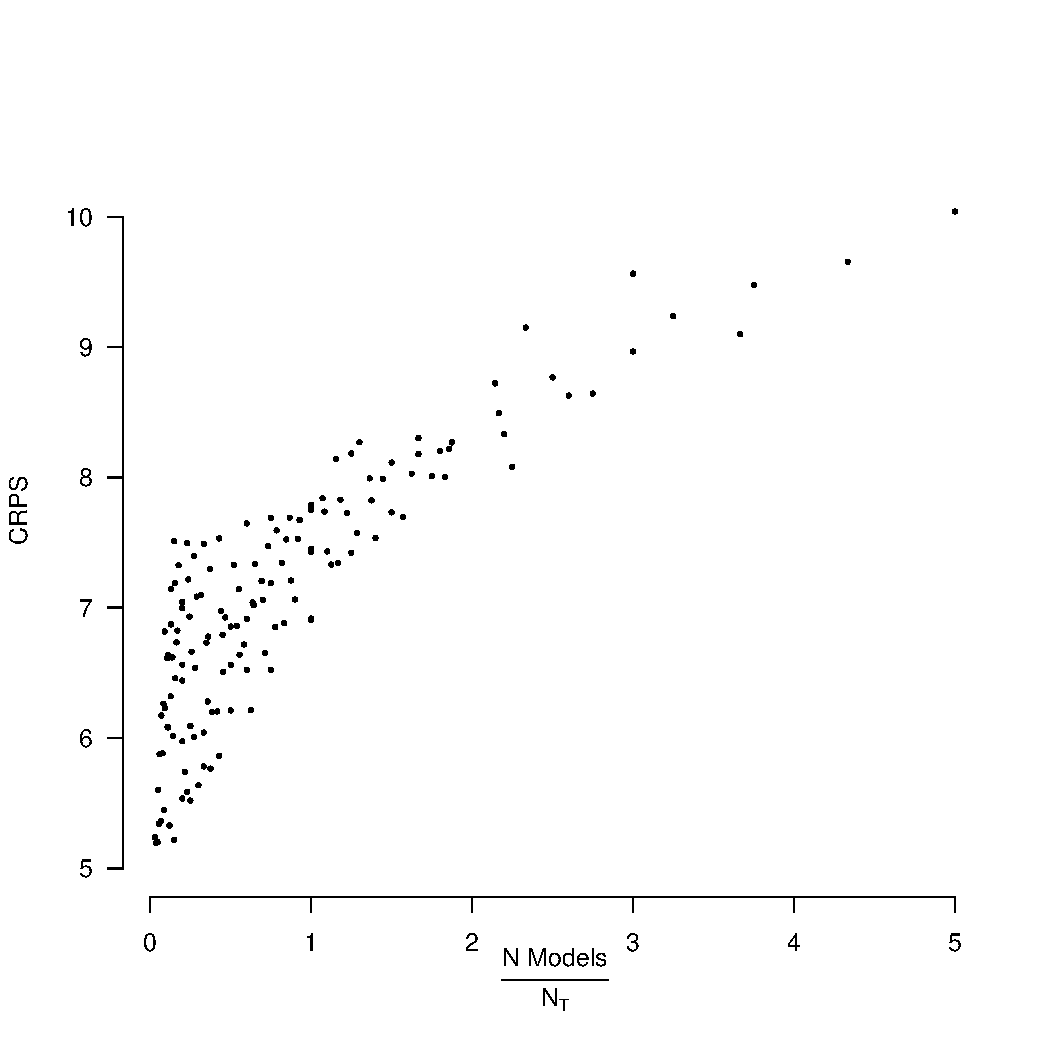
\includegraphics[scale=.5]{2D}
\end{figure}

Figure~\ref{simplot1} shows how the out-of-sample performance of the
EBMA method, as measured by CRPS against the ratio of the number of
component models included and the size of the calibration period
($\frac{K}{n_T}$). As one can see, the performance of the EBMA model
depends significantly on this ratio. As the number of forecast models
included as components increases, or the calibration sample size
decreases, CRPS rises.  That is, the predictive performance of the
ensembles decreases as a function of $\frac{K}{n_T}$.

Thinking of each parameter in isolation, the predictive power of the
EBMA model decreases as the number of components in the true data
generating process increases. That is, as the number of model
parameters that \textit{must} be correctly estimated to make accurate
predictions increases, the quality of the forecast goes down. Second,
CRPS is a decreasing function of $n_{T}$, i.e. the performance of the
baseline EBMA model improves as the calibration sample
grows.\footnote{Examining each parameter in isolation supports this
  claim, although the relationship his highly interactive (results not
  shown).}

%Second, Figure~\ref{simplot1} shows out-of-sample CRPS when $n_T=5$
%(black), $n_T=11$ (blue), and $n_T=100$ (red).  For all values of $k$,
%the CRPS is a decreasing function of $n_T$.  This illustrates that the
%performance of the baseline EBMA model improves as the calibration
%sample grows.

%\begin{figure}[ht]
%\caption{A plot to show that $c$ helps in some situations}
%\label{simplot2}
%\centering
%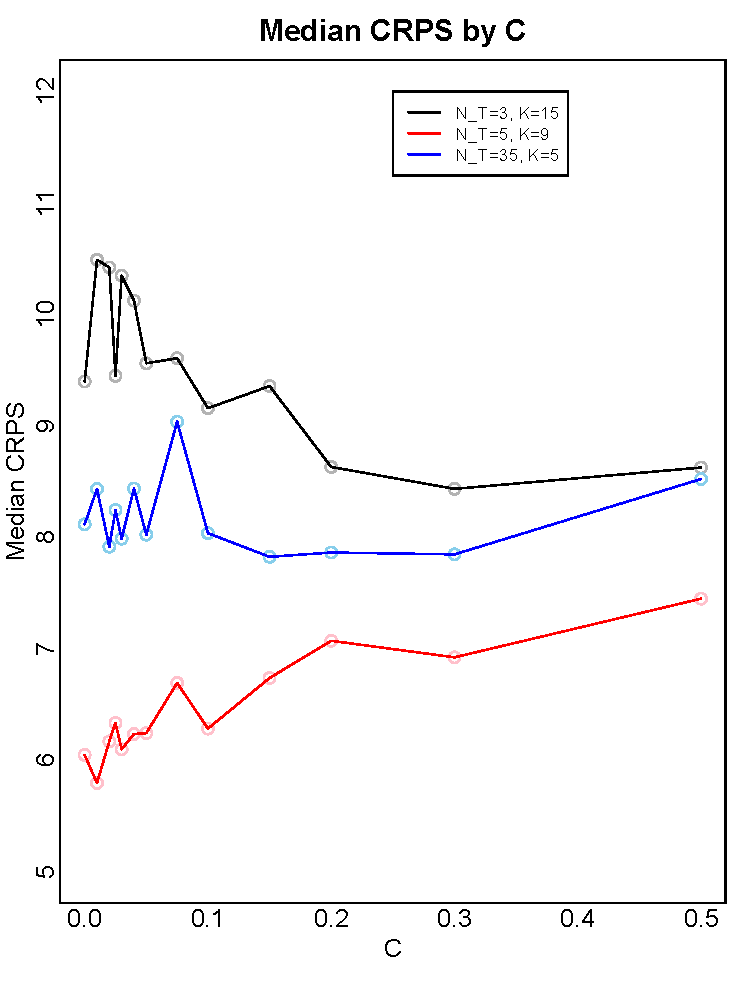
\includegraphics[scale=.8]{SimTemp2}
%\end{figure}

\begin{figure}[ht]
\caption{CRPS with ``Wisdom of Crowds'' Parameter}
\label{3d}
\centering
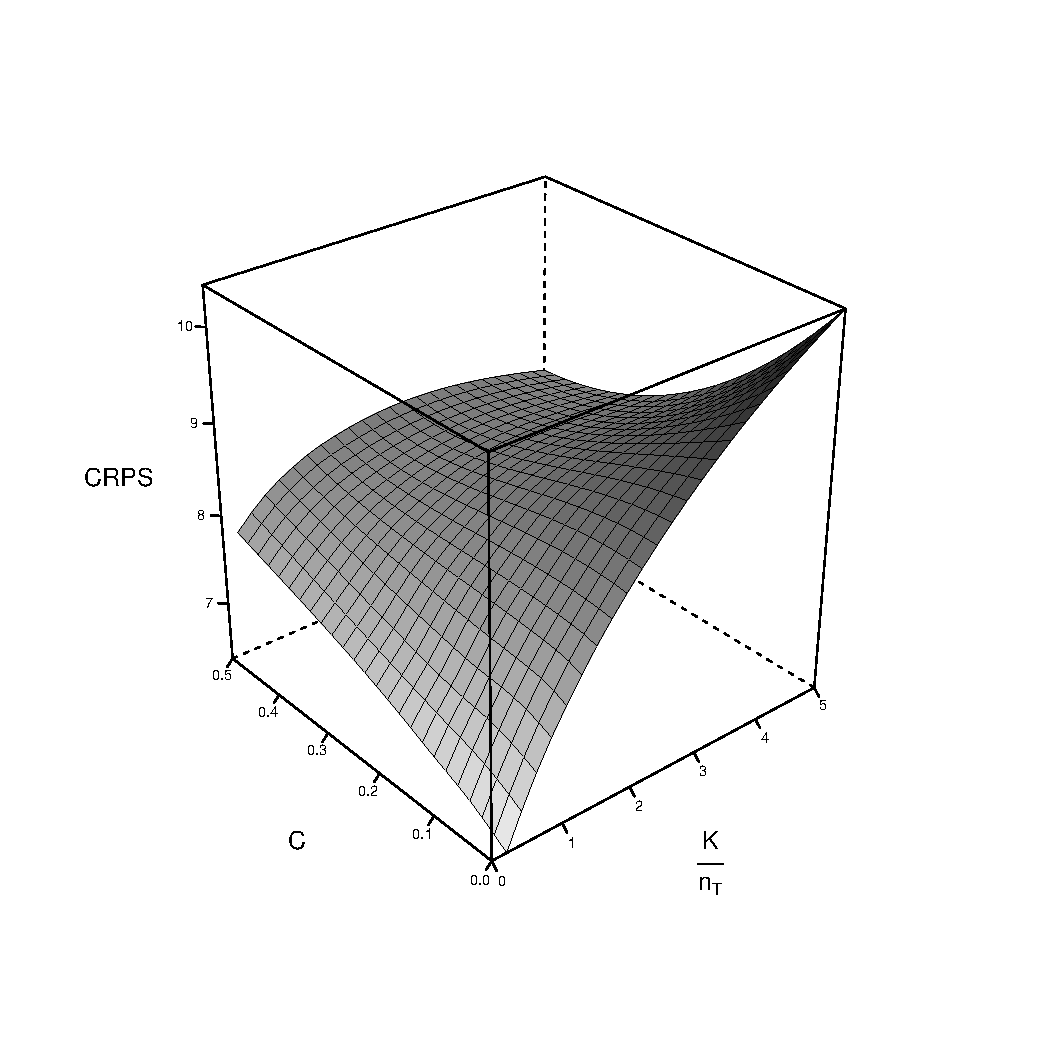
\includegraphics[scale=.6]{3D}
\end{figure}

The remaining question, then, is to what degree adding the ``wisdom of
crowds'' parameter to the baseline model improves performance.  To
answer, we examined the out-of-sample predictive performance of EBMA
for differing values of $c$.  Figure~\ref{3d} shows a smoothed plot of
the median CRPS for differing values of the ratio $\frac{K}{n_T}$ and
$c$ in our simulation. Darker gray tones depict higher CRPS
levels. The plot shows that while CRPS generally still increases with
higher values of $\frac{K}{n_T}$, including a ``wisdom of crowds''
parameter within the EBMA algorithm can help when $\frac{K}{n_T}$ is
large.


There are two aspects of Figure~\ref{3d} that are particularly
salient.  First, note that the addition of $c$ to the base EBMA model
does not uniformly aid in out-of-sample performance.  When the
calibration sample is modestly large and there are few models to
calibrate, the addition of $c$ uniformly decreases model performance.
However, with small calibration samples and modestly large numbers of
component models, the addition of $c$ aids predictive
performance. Second, the relationship between $c$ and CRPS is
non-monotonic.  CRPS decreases for small to modest values of $c$, but
eventually begins to rise.  While this is far from a complete analysis
of the simulated data, it does serve the limited purposes of
demonstrating that, in some circumstances, the ``wisdom of crowds''
parameter aids prediction under some circumstances.

Generally speaking, in choosing $c$ the researcher faces a trade-off
between possible overweighting certain models based on the performance
in short calibration periods and moving too far into the direction of
a simple average. A relatively small $c$ seems to generally aid
performance.  Based on our examination of the broader set of
simulations, we generally recommend the selection of values of $c \in
[0, 0.1]$. The simulations favor small values of $c$ as the ratio of
$K$ to $n_T$ decreases.  In our experience based on the simulations,
as well as cross-validation studies during the applications presented
below, we feel a $c$ value at $0.05$ a good default choice, although
the ``best'' value of $c$ may vary from application to application.
It may be preferable to many researchers to choose the value of $c$
based on a k-fold cross-validation study of the calibration sample.

Bearing these results in mind, we now turn to examining how these
methods work in two areas that exemplify forecasting in the social
sciences. The first is the prediction of unemployment in the United
States, and the second is predicting the vote for the incumbent-party
candidate in U.S. presidential elections. Both areas have well
developed forecasting traditions in the scholarly and policy
community.


\subsection{Quarterly unemployment in the United States}
\label{econ}

Forecasting macroeconomic variables is a quite common exercise in the
field of economics and statistics. Policy makers and businesses both
have enormous interest in the calculation of accurate forecasts of
economic variables. These forecasts are often created using a wide
variety of statistical models, however often professional forecast are
based only on expert knowledge.\footnote{For a more comprehensive
  overview on foresting of economic variables and time-series
  forecasting see \citet{Elliott:Timmermann:2008} and
  \citet{Goijer:Hyndman:2006}.}  The majority of scholars employ
time-series models, most commonly applying autoregressive integrated
moving average (ARIMA) and vector autoregressive (VAR) models. The
sophistication and complexity of forecasting models has increased
considerably over time. In particular, non-linear dynamic models have
gained prominence including threshold autoregressive models, Markov
switching autoregressive models and smooth transition autoregression
\citep{Elliott:Timmermann:2008,Montgomery:etal:1998}. More recently,
forecasters have added Bayesian VAR models and state-space models to
their arsenal \citep{Goijer:Hyndman:2006,Elliott:Timmermann:2008}.

Unsurprisingly, given the large number of ongoing forecasts, scholars
have attempted to improve predictive accuracy by combining forecasts
\citep{Bates:1969, Palm:Zellner:1992, Elliott:Timmermann:2008}.
Recently, EBMA and related Bayesian model averaging methods have been
successfully employed to create ensemble forecasts of various
macroeconomic indicators including inflation
\citep{Koop:2010,Wright:2009}, GDP \citep{Billio:2010}, stock prices
\citep{Billio:2011}, and exchange rates \citep{Wright:2008}.

Policy makers too have come to rely on ensemble forecasts of a sort.
The desire to aggregate the collective wisdom of multiple forecasting
teams is apparent in the \textit{Survey of Professional Forecasters
  (SPF)} published by the \textit{Federal Reserve Bank of
  Philadelphia}.  The \textit{SPF} includes forecasts for a large
number of macroeconomic variables in the U.S., including the
unemployment rate, inflation, and GDP growth.\footnote{The
  \textit{SPF} was first administered in 1968 by the American
  Statistical Association and the National Bureau of Economic Research
  (NBER).  Since 1990, however, it is run by the Federal Reserve Bank
  of Philadelphia.
  \url{http://www.phil.frb.org/research-and-data/real-time-center/survey-of-professional-forecasters/}}
In the first month of every quarter, a survey is sent to selected
forecasters and is returned by the middle of the second month of the
quarter. Forecasts are made for the current quarter as well as several
quarters into the future, and a significant amount of attention is
given to the average (usually the median) reported forecast.

This plethora of predictions seems ideal for applying EBMA.
Nonetheless, it is plagued by the same issues as discussed in
Section~\ref{theproblem}.  Even with quarterly measures, there are
relatively few observations, many forecasting teams, and a significant
number of missing observations.  This setting, therefore, provides a
test bed for the adjusted EBMA model discussed above.

We focus on forecasting the civilian unemployment rate (UNEMP) as
published by the \textit{SPF}. For this application, we selected the
forecast horizon to be four quarters into the future, i.e. predictions
made in the first quarter of 2002 are for the first quarter of 2003
and so on. In total, the \textit{SPF} data on unemployment contains
forecasts by 569 different teams. However, for any quarter, the
average number of teams making a prediction for four quarters into the
future is quite small and the majority of observations for any given
quarter are missing.\footnote{On average only 8.4 per cent of all
  teams make a forecast for any one quarter.}

To provide a meaningful benchmark for our adjusted EBMA model, we also
include the ``Green Book'' forecasts produced by the Federal Reserve
in the ensemble. These forecasts are made by the research staff of the
Board of Governors and are handed out prior to meetings of the Federal
Reserve Open Market Committee (FOMC).\footnote{One issue with forecast
  evaluation in many domains in economics is that the macroeconomic
  data (i.e. our ``true observations'') are revised regularly. The
  unemployment rate for a given quarter at that time is generally an
  estimate that is subject to revision when better data becomes
  available. When evaluating forecasts, it is thus important whether
  predictions are compared to the outcome data for each quarter
  available at the time or whether the revised and most recent data is
  used. As \citet{Croushore:Stark:2001} describe, depending on the
  forecast exercise, it can make a difference whether the forecast
  models are evaluated using ``real-time'' (original estimate) or the
  ``latest available'' (revised) data. We have decided here to use the
  ``latest available'' data and do not believe that this choice
  affects our results, as all predictions are evaluated against the
  same data and EBMA is a mixture of the component forecast
  models. Thus the component models and our benchmark model are
  estimated and evaluated on the same
  data.} %However, in a future version of this paper we will
  %replicate this analysis using real-time data to evaluate the
  %forecasts.} % DO WE WANT TO DO THAT BEFORE SUBMISSION?

Taking the \textit{SPF} and Green Book unemployment forecasts, we
calibrate an ensemble model for each period $t$, using forecaster
performance over the past ten quarters.  Only forecasts that had made
predictions for five of these quarters were included in the ensemble.
Thus, the EBMA model uses only 163 models out of a possible 293
forecasting models that made predictions during the period we study.
Due to missing data early in the time series, and the fact that Green
Book forecasts are sequestered for five years, we generate forecasts
beginning in the third quarter of 1983 and running through the fourth
quarter of 2007.



\begin{figure}[h]
\caption{Observed and forecasted U.S. unemployment (1981-2007)}
\label{timeSeries}
\begin{center}
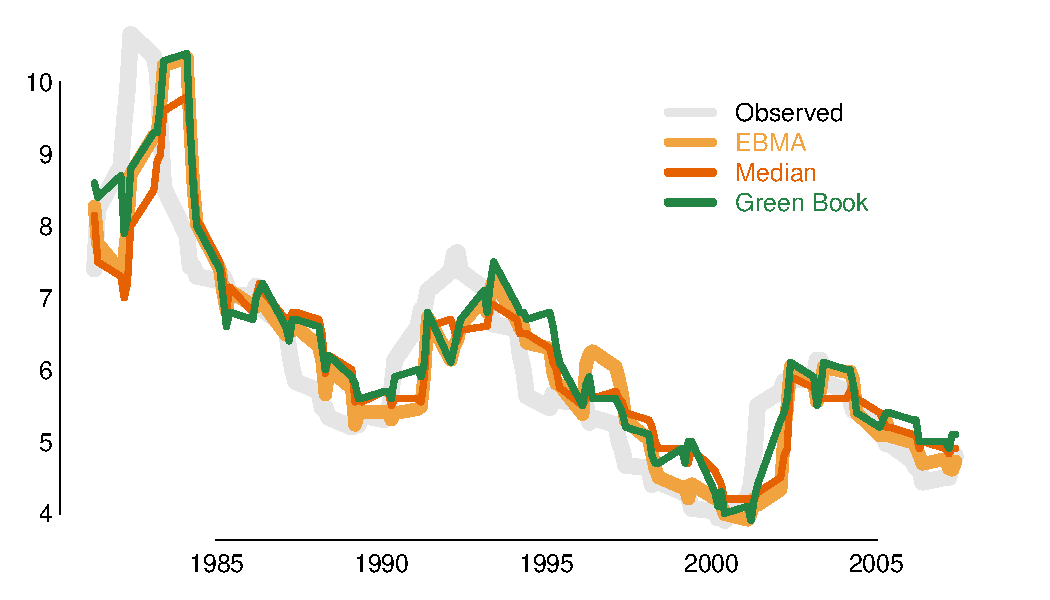
\includegraphics[scale=.8]{mdwtimeSeries2}
\end{center}
\end{figure}


One approach to evaluating the performance of EBMA is to compare its
predictive accuracy to that made by other systematic forecasting
efforts and methods of generating ensemble predictions.  Specifically,
we compare EBMA's ($c=0.05$) predictive accuracy to (1) the Green
Book, (2) the median forecaster prediction and (3) the mean forecaster
prediction.\footnote{Note that the EBMA model is calculated on only a
  the subset of forecasts that have made a sufficiently large number
  of recent predictions to calibrate model weights.  Thus, the median
  forecast and the ensemble forecast will not be the same even when
  $c=1$.} 

Figure~\ref{timeSeries} shows a visual representation of the
Greenbook, median SPF and the EBMA (with $c=0.05$) forecasts over
time, as well as the true unemployment rate. As was noted above and is
clearly visible, the SPF and Greenbook forecasts are quite
similar. \citet{Baghestani:2008} noted that the Greenbook forecast is
slightly biased to over predict the unemployment rate. In some periods
EBMA is able to correct this bias, however given the similarity of
component models, the improvement in that direction is rather
small. In general, however, it is easily visible that the EBMA
forecast is closer to the actual rate than the median SPF or the Green
Book forecast.

\begin{table}[h]
\caption{Comparing adjusted EBMA models with Green Book, median, and mean forecasts of U.S. Unemployment (1981-2007)}
\begin{center}
\begin{tabular}{lrrrrrrrr}
\toprule
 & MAE & RMSE & MAD & RMSLE & MAPE & MEAPE & MRAE & PW \\ 
\midrule
 EBMA (c=0)& 0.54 & 0.74 & 0.37 & 0.093 & 8.37 & 6.49 & \textbf{0.73} & \textbf{27.36} \\ 
  EBMA (c=0.05)& \textbf{0.54} & 0.74 &\textbf{ 0.37} & \textbf{0.093} & \textbf{8.33} & \textbf{6.30} & 0.75 & \textbf{27.36} \\ 
 EBMA (c=0.1)& 0.54 & 0.74 & 0.35 & 0.093 & 8.40 & 6.44 & 0.76 & 28.30 \\ 
EBMA (c=1) & 0.61 & 0.80 & 0.46 & 0.102 & 9.72 & 8.92 & 0.95 & 46.23 \\ 
 Green Book& 0.57 & \textbf{0.73} & 0.43 & 0.093 & 9.37 & 8.81 & 1.00 & 45.28 \\ 
 Forecast Median& 0.62 & 0.81 & 0.47 & 0.103 & 9.83 & 8.87 & 0.98 & 47.17 \\ 
Forecast Mean& 0.61 & 0.80 & 0.46 & 0.102 & 9.71 & 9.06 & 0.93 & 46.23 \\ 
\bottomrule
\end{tabular}
\end{center}

%FH: WE SHOULD ADD CRPS HERE? SINCE WE ADVOCATE IT SO STRONGLY ABOVE
%JMM: WE CANNOT CALCULATE FOR GREEEN BOOK, MEDIAN, AND MEAN

\label{compareTable1}
Definitions of model fit statistics are provided in the Appendix. The model with the lowest score for each metric are shown in bold.  Differences between model performance may not be obvious due to rounding.
\end{table}


Table~\ref{compareTable1} formally compares these baseline models to
EBMA models with $c=$0, 0.05, 0.1, and 1 respectively.  To do this, we
focus on eight model fit indices available in the literature
\citep{brandt:freeman:schrodt:2011}.\footnote{We are unable to use
  CRPS here because we do not have the predictive PDFs for the Green
  Book, SPF Mean, or SPF Median models.}  The eight metrics we use are
mean absolute error (MAE), root mean squared error (RMSE), median
absolute deviation (MAD), root mean squared logarithmic error (RMSLE),
mean absolute percentage error (MAPE), median absolute percentage
error (MEAPE), median relative absolute error (MRAE) and percent worse
(PW).  The latter two metrics are measured relative to a naive model,
simply predicting the future rate of unemployment as being the same as
the current rate of unemployment.  Further details for these metrics
are shown the Appendix B.


The bolded cells in each column of Table~\ref{compareTable1} indicate
the model that performed ``best'' as measured by each metric.  With
one exception, (the Green Book outperforms the ensemble by 0.01 on
RMSE), the EBMA model outperforms both the Green Book forecast and the
unweighted mean and median forecast on every metric.  Moreover, these
results confirm that the $c$ parameter is best set to a small number.
In general, the model with $c=0.05$ performs best (or is tied for
best) on six out of eight of these metrics.


% \begin{figure}[!htb]
%   \caption{Ensemble weights for SPF forecasts of U.S. unemployment
%     with a rolling calibration window}
% \label{modelWeights}
% \begin{center}
% 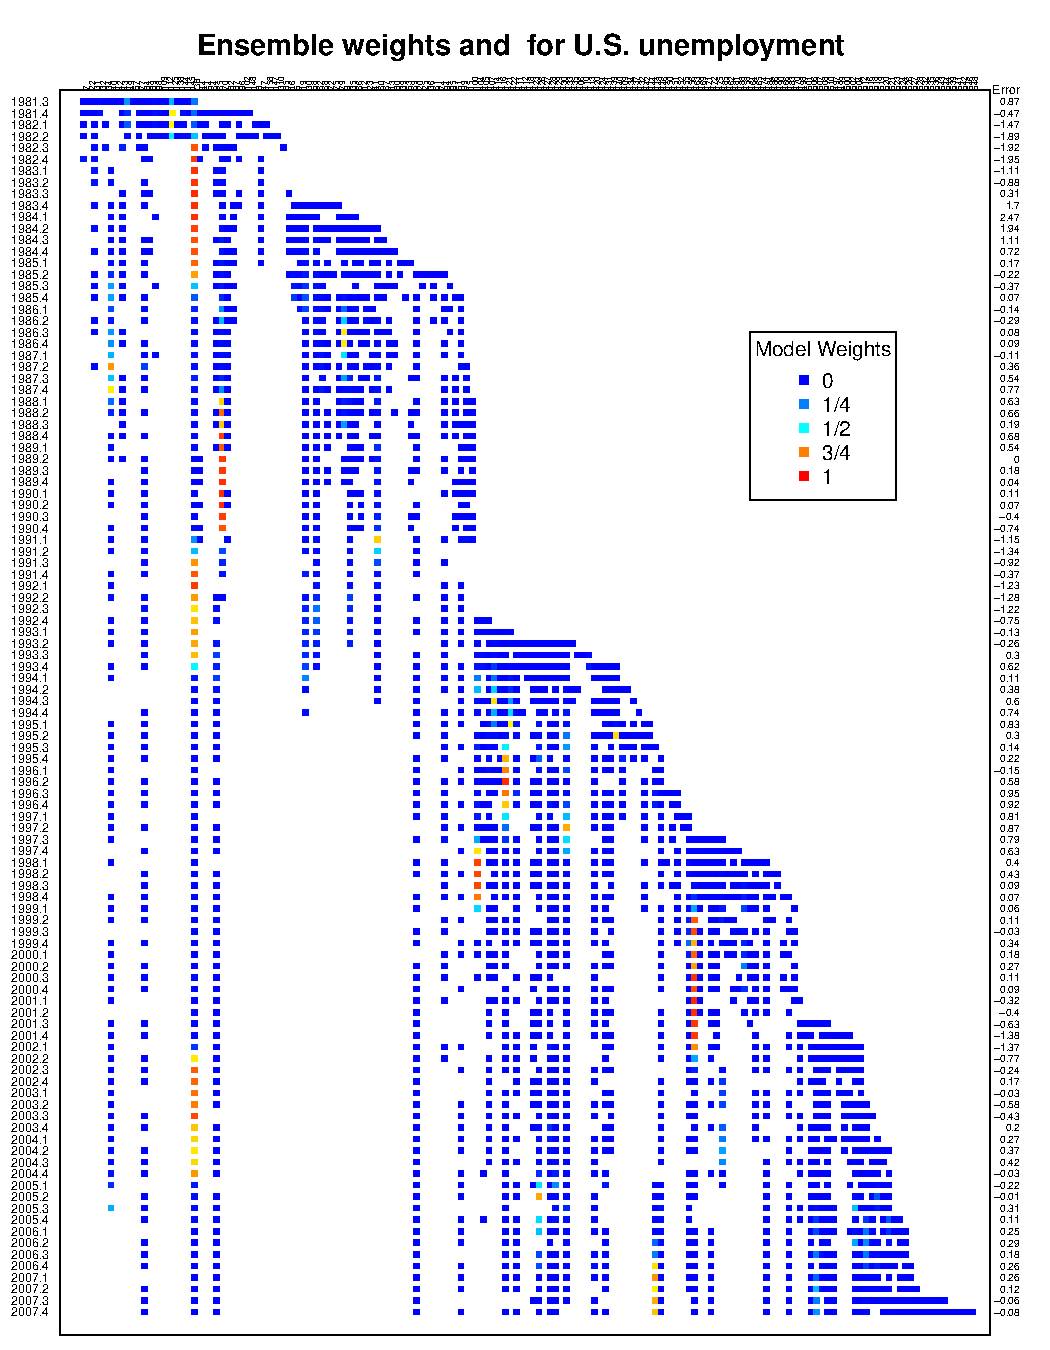
\includegraphics[scale=.70]{awesome}
% \end{center}

% \footnotesize This graphic illustrates the component weights for each EBMA
% model estimated between 1983 and 2007. Ensembles are calibrated on the
% past ten quarters. The colors range from blue to red to indicate
% increasing weights for components in a given ensemble model. Those
% components excluded in a given model are missing.

% \end{figure}

% Figure~\ref{modelWeights} provides a visual representation of EBMA
% model calibrations throughout this period.  In this figure, the wisdom
% of crowds tuning parameter is set to a modest $c=0.05$.  The colors
% indicate the model weight assigned to each component on a red-blue
% color ramp (components not included in the ensemble are blank).
% Models assigned no weight are shown in dark blue while models that are
% heavily weighted are shown in red. Figure~\ref{modelWeights} also
% illustrates the difficulties inherent in forecasting with this type of
% data.  For any given year, only a subset of forecasting teams offer a
% prediction.  Further, an even smaller subset contains models that both
% offer a prediction and have made a sufficiently large number of prior
% forecasts to facilitate model calibration.  Finally, the very
% sparseness of the data encourages the ensemble model to place a very
% large amount of weight on the best performing models.



%\begin{figure}[!htb]
%\caption{Comparing predictive accuracy of EBMA and component models with eight metrics}
%\label{compare2Components}
%\begin{center}
%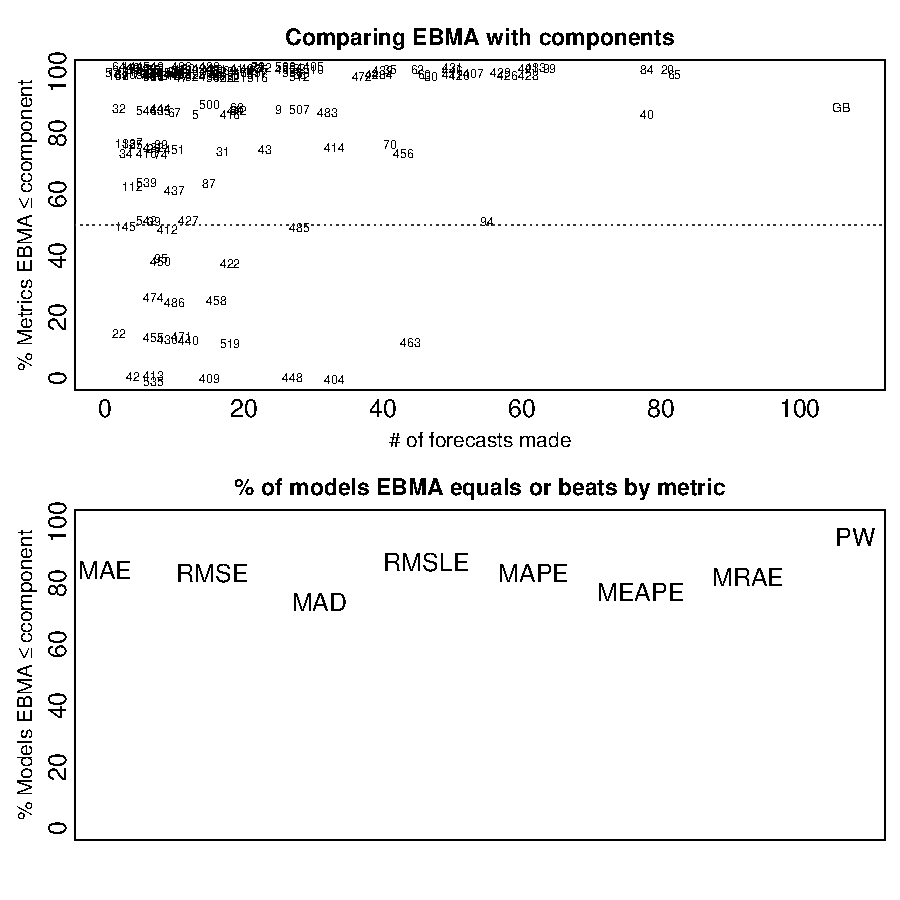
\includegraphics{compare2Components}
%\end{center}
%
%\footnotesize
%The top panel plots EBMA's relative performance, as measured by eight
%forecasting metrics, to each of its components against the number of
%forecasts generated by the component models.  The bottom panel shows
%the percentage of component models that EBMA matches or outperforms as
%measured by each metric.  Details on the eight forecasting metrics are
%shown in the Appendix.  The Green Book forecast is labeled (GB) and is
%located in the upper left portion of the top panel).
%
%
%\end{figure}

% latex table generated in R 2.15.2 by xtable 1.7-0 package
% Thu Feb  7 15:10:56 2013
\begin{table}[ht]
\begin{center}
\caption{Comparing predictive accuracy of EBMA and component models with eight metrics}
\begin{tabular}{rrrrr}
  \toprule
  % \multicolumn{5}{c}{Number of Predictions Made}\\
 & 1 --10& 11-30 & 31--60 & $>60$ \\ 
  \midrule
7 -- 8 & 0.20 & 0.33 & 0.10 & 0.04 \\ 
 5 -- 6  & 0.04 & 0.04 & 0.03 & 0.01 \\ 
 2 -- 4 & 0.02 & 0.03 & 0.01 & 0.00 \\ 
 0 -- 1 & 0.08 & 0.04 & 0.01 & 0.00 \\ 
   \bottomrule
\end{tabular}
\end{center}
\label{compareTable2}
The table shows EBMA's relative performance, as measured by eight forecasting metrics, to each of its components against the number of forecasts generated by the individual component models.  
Rows show the number of metrics EBMA scores better on than the respective component models, while the columns show the number of predictions made by these models. 
\end{table}



We now turn to evaluating the performance of the ensemble relative to
its 163 component forecasts.  It is important to note that many of
these forecasters make predictions in a relatively small subset of
cases.  That is, each model $k$ offers forecasts for only a subset of
cases $n_k \subset n$.  To create a fair comparison, therefore, we
calculate these fit indices only for $n_k \forall k \in [1,K]$.  By
this measure, the EBMA model performs very well.
Table~\ref{compareTable2} provides a summary of these results.  The
rows of the table show the number of metrics by which EBMA outperforms
components in each column, while columns show the number of forecasts
made by these models. The table is filled with the share of the total
number of component models falling into each cell. Thus, the values
in all of the cell will sum to unity. For instance, the top-left cell
represents cases where EBMA is better on at least 7 out of eight
metrics for component models making between 1 and 10 predictions.
Approximately 20\% of models belong in this category.

Notably, the relative superiority of EBMA to its components is
somewhat less for components that provide few forecasts.  This
reflects the fact that with so many forecasts, some are likely to be
more accurate than the ensemble by chance alone. Additionally, when
the number of forecasts is low it is likely that a given model
received less weight than it ``deserves'' given the model's
performance.\footnote{See Appendix A for a discussion of how EBMA
  handles missing component forecasts.} However,
Table~\ref{compareTable2}, shows that, across a large number of
forecasts, EBMA significantly outperforms any of its components.  That
is, when moving to the right in the table the values in the lower
cells decrease. It is also worth noting that only 6 out of the total
163 components outperforms EBMA on every metric.




\subsection{U.S. presidential elections}

We now turn to the task of combining expert predictions of
U.S. presidential elections.\footnote{See also,
  \citet{Montgomery:2012c}.}  This example provides a clear
illustration of the difficulties of creating ensemble forecasts in the
social sciences and allows us to further illustrate the advantages of
generating predictive PDFs when focusing on a limited number of
important events.

Predicting U.S. presidential elections is, perhaps, the quintissential
forecasting task that combines all of the issues discussed in
Section~\ref{theproblem}.  Table~\ref{tab:one} represents nearly the
entirety of scholarly forecasts which produced more than one true
out-of-sample forecast for elections in the 20th century prior to the
2012 election.\footnote{ See, for example \citet[][]{Fair:2009,
    Fair2011, Abramowitz:2008, Campbell:2008,
    Cuzan:2004,Cuzan:Bundrick:2008,hibbs:2012, Lockerbie:2008,
    Erikson:Wlezien:2008, Graefe:2010, Holbrook:2008}.  A recent
  symposium in {\em PS: Political Science \& Politics} presents and
  summarizes attempts by a variety of scholars to predict the 2012
  U.S. presidential election. In a symposium contribution, we use the
  in-sample fitted values of the election forecasting models to
  calibrate the EBMA model \citep{Montgomery:2012c}. However, the
  strength of EBMA is greatest when the model is calibrated on true
  out-of-sample forecasts as we do here.}  In this instance, we have
only five observations by which to calibrate an ensemble model, while
we have nine forecasting models.  Moreover, several of the individual
forecasts are missing for a significant portion of the data.  The
forecast of Cuz\`an, for instance, is missing for 60\% of the
elections in this dataset.\footnote{The predictions by Cuz\`an for
  2004 stems from the FISCAL model published prior to the 2004
  election by \citet{Cuzan:2004}, while the 2008 prediction comes from
  the FPRIME short model presented in advance of the election
  \citep{Cuzan:Bundrick:2008}. However, both models are quite similar
  in their composition.}

\begin{table}[ht]
\caption{Pre-election forecasts of the percent of the two-party vote going to the incumbent party in U.S. Presidential elections}
\label{tab:one}
\footnotesize
% latex table generated in R 2.15.2 by xtable 1.7-0 package
% Tue Jan 29 13:42:53 2013
\begin{center}
\begin{tabular}{rrrrrrrrrrrr}
  \toprule
 & Year & F & A & C & H & LBRT & L & Hol & EW & Cuz  \\ 
  \midrule
1 & 1992 & 55.70 & 46.30 & 47.10 & 48.90 &  &  &  &  &   \\ 
  2 & 1996 & 49.50 & 56.80 & 58.10 & 53.50 & 54.80 &  & 57.20 & 57.20 &   \\ 
  3 & 2000 & 50.80 & 53.20 & 52.80 & 53.80 & 55.40 & 60.30 & 60.30 & 55.20 &   \\ 
  4 & 2004 & 57.50 & 53.70 & 53.80 & 53.20 & 49.90 & 57.60 & 54.50 & 52.30 & 52.80  \\ 
  5 & 2008 & 48.10 & 45.70 & 52.70 & 48.20 & 49.90 & 41.80 & 44.30 & 47.80 & 48.00  \\ 
   \bottomrule
%\begin{center}
%\begin{tabular}{rlrrrrrrrrr}
%  \toprule
%  & F & A & C & H & LBRT & L & Hol & EW & Cuz \\ 
%  \midrule
%  1992 & 55.7 & 46.3 & 49.7 & 48.9 & 47.3 &  &  &  &  \\ 
%  1996 & 49.5 & 57.0 & 55.5 & 53.5 & 53.3 &  & 57.2 & 55.6 &  \\ 
%  2000 & 50.8 & 53.2 & 52.8 & 53.8 & 55.4 & 60.3 & 60.3 & 55.2 &  \\ 
%  2004 & 57.5 & 53.7 & 52.8 & 53.2 & 49.9 & 57.6 & 55.8 & 52.9 & 51.1 \\ 
%  2008 & 48.1 & 45.7 & 52.7 & 48.5 & 43.4 & 41.8 & 44.3 & 47.8 & 48.1 \\ 
%  \bottomrule
%
\end{tabular}
\end{center}
Forecasts were published prior to each election by \textbf{F}air, \textbf{A}bramowitz, \textbf{C}ampbell, \textbf{H}ibbs, \textbf{L}ewis-\textbf{B}eck and \textbf{R}ice (1992), Lewis-Beck and \textbf{T}ien  (1996-2008),   \textbf{L}ockerbie, \textbf{Hol}brook, \textbf{E}rikson and \textbf{W}lezien and \textbf{Cuz}\`an and Bundrick. 
\end{table}


Using the forecasts shown in Table~\ref{tab:one},\footnote{The
  out-of-sample predictions for these models were collected from the
  individual journal articles, personal websites and symposia
  introductions. When multiple forecasts were made we used the
  authors' preferred forecast, or took the mean if no preference was
  given
  \citep{Hibbs:1992,Holbrook:1996,LewisBeckTien:1996,EriksonWlezien:1996,Abramowitz:2000,Hibbs:2000,CampbellGarand:2000,Campbell:2000,Campbell:2001,Hibbs:2004,Campbell:2004,Campbell:2005,Campbell:2008a,Abramowitz:2012,Campbell:2012,Cuzan:2012,EriksonWlezien:2012,Fair:2012,Hibbs:2012a,Holbrook:2012,LewisBeckTien:2012,Lockerbie:2012}.}
we fit an EBMA model with $c=0.05$.  The model weights and in-sample
fit statistics for the ensemble and its components are shown in
Table~\ref{presModel}.  As can be seen, the EBMA model assigns the
majority of weight to the Abramowitz model with the model by Hibbs
receiving the second largest weight. These weights are based on the
performance of each model in forecasting the incumbent vote share in
the presidential elections between 1992 and 2008. The Cuz\`an and
Bundrick model is weighted to such a small degree because only
out-of-sample predictions for 2004 and 2008 were available.


% latex table generated in R 2.15.1 by xtable 1.7-0 package
% Sun Aug 12 21:58:55 2012
\begin{table}[ht]
\caption{Model weights and in-sample fit statistics for EBMA model of U.S. Presidential Elections (1992-2008)}
\label{presModel}
\begin{center}
\begin{tabular}{lrrrr}
  \toprule
 & \shortstack{EBMA\\ Weight}&RMSE &MAE \\ 
  \midrule
  EBMA &  & 1.92 & 1.49 \\ 
  Fair & 0.02 & 5.53 & 4.58 \\ 
  Abramowitz & 0.80 & 1.98 & 1.68 \\ 
  Campbell & 0.02 & 3.63 & 3.08 \\ 
  Hibbs & 0.06 & 2.31 & 2.18 \\ 
  Lewis-Beck, Rice, and Tien  & 0.06 & 2.87 & 2.16 \\ 
  Lockerbie & 0.00 & 7.33 & 6.97 \\ 
  Holbrook & 0.01 & 5.50 & 4.45 \\ 
  Erikson and Wlezien  & 0.02 & 2.90 & 2.50 \\ 
  Cuz\`an	 & 0.00 & 1.65 & 1.65 \\ 
  
%EBMA &  & 1.92 & 1.56 \\ 
%  Fair & 0.02 & 5.53 & 4.58 \\ 
%  Abramowitz & 0.78 & 2.02 & 1.72 \\ 
%  Campbell  & 0.07 & 3.46 & 2.88 \\ 
%  Hibbs  & 0.04 & 2.68 & 2.44 \\ 
%  Lewis-Beck, Rice, and Tien & 0.06 & 2.78 & 2.28 \\ 
%  Lockerbie  & 0.00 & 7.33 & 6.97 \\ 
% Holbrook & 0.01 & 5.73 & 4.77 \\ 
%  Erikson and Wlezien & 0.02 & 2.74 & 2.25 \\ 
%  Cuz\`an & 0.00 & 1.27 & 0.95 \\ 
   \bottomrule
\end{tabular}
\end{center}
\end{table}


Figure~\ref{pres} shows the posterior predictive distribution for the
2008 election (top) and, based on the forecasts from each of the
component models, the 2012 election.  Component models' predictive
distributions are shown in color (scaled by their respective weight),
while the EBMA predictive distribution is shown in black, the bold
dash displays the point prediction for the EBMA model. The vertical
dashed line depicts the actual election results in 2008 and 2012.

\begin{figure}[h]
\caption{Predictive ensemble PDFs of incumbent-part vote share in U.S. Presidential Elections}
\label{pres}
\begin{center}
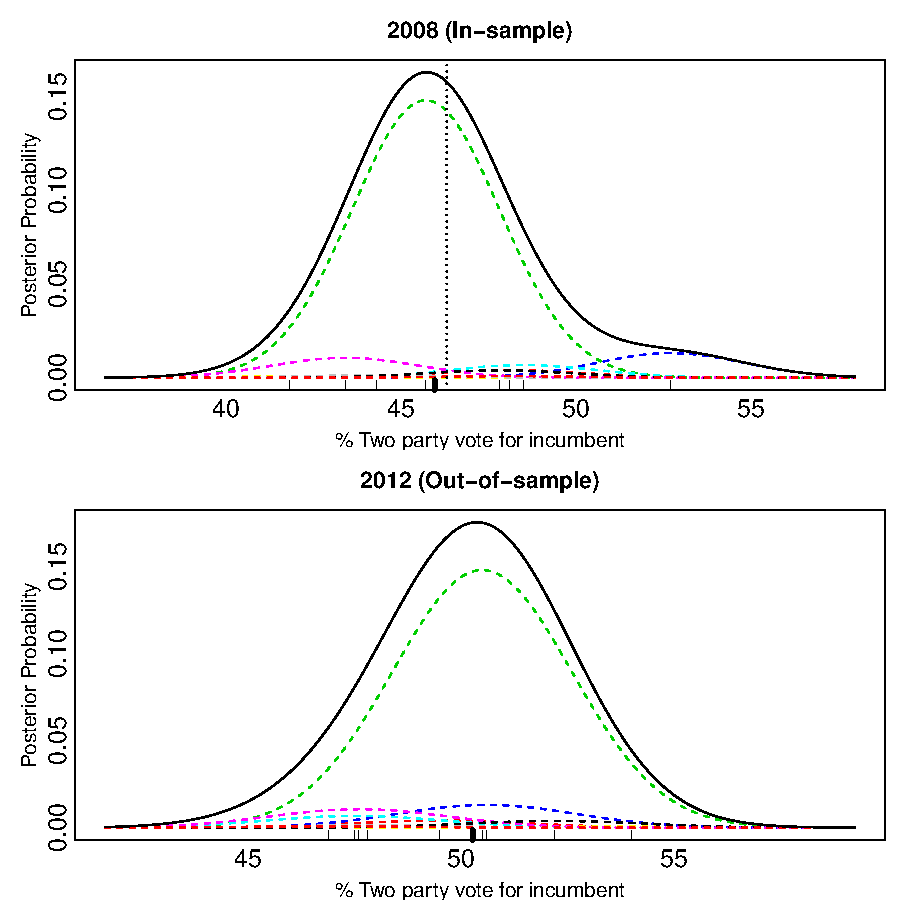
\includegraphics[scale=.8]{presForecast}
\end{center}
The figure shows the density functions for each of the component
models in different colors and scaled by their respective weight. The black curve is the density of the EBMA
prediction, with the bold dash indicating the EBMA point
prediction. The vertical dashed lines show the actual result of the 2008 and 2012 elections.
\end{figure}


The EBMA model ($c=0.05$) predicted 50.3\% of the two-party vote share
for Obama in 2012.  This resulted in a reasonably large absolute error of
1.7\%.\footnote{The EBMA model assigned considerable weight to models
  predicting a Romney \textit{victory}, especially \citet{Hibbs:2012a}
  and \citet{LewisBeckTien:2012}.}  Figure~\ref{pres} shows that the
EBMA prediction performs better than the majority of component
forecasts for the 2012 election, with only three providing a more
accurate estimate. However, we believe it is important to note that
this it is difficult to evaluate EBMA against its components using
just one out-of-sample observation.

% latex table generated in R 2.15.2 by xtable 1.7-0 package
% Tue Jan 29 15:05:47 2013
\begin{table}[ht]
\caption{Comparing Model Results for U.S. Presidential Elections 2012}
\label{presModel12}
\begin{center}
\begin{tabular}{rrrrrr}
  \toprule
 & Mean & Median & EBMA ($c=0$) & EBMA ($c=0.05$) & EBMA ($c=0.1$) \\ 
  \midrule
2012 prediction & 49.9 & 49.5 & 49 & 50.3 & 50.1 \\ 
  Absolute Error & 2 & 2.4 & 2.9 & 1.6 & 1.8 \\ 
   \bottomrule
\end{tabular}
\end{center}
\end{table}

A more important comparison is to examine how EBMA performs versus
other methods of aggregating forecasts for the 2012 election.
Table~\ref{presModel12} shows the point predictions and absolute
errors associated with the simple arithmetic mean, the median, and
EBMA models fit with $c=0$, $c=0.05$, and $c=0.1$.  While the
differences in model weights are relatively small, the EBMA prediction
for 2012 was 49\% and 50.1\% for and EBMA model with $c=0$ and $c=0.1$
respectively -- both considerably worse than the prediction with
$c=0.05$.

EBMA with a ``wisdom of crowds'' parameter of $0.05$ also did
considerably better relative to naive approaches to aggregation. The simple
arithmetic average of the component models' predictions was 49.9\% and
the median prediction was 49.5\%. In essence, while we believe
prediction methods should be evaluated on more than one observation,
this example again signifies the utility of EBMA in forecasting tasks
and in particular the improvements the ``wisdom of crowds'' parameter
offers to out-of-sample predictions in the context of sparse data.


\section{Discussion} 
Ensemble Bayesian model averaging is a principled way of combining
forecasts to improve prediction accuracy. However, the calibration of
such models in the social sciences is often hindered by the quality as
well as availability of data. For one, in many forecasting exercises
the number of forecasting models is large, yet the number of
observations on which the EBMA model can be trained is small. This
creates problems for the estimation of model weights, as it is likely
that overly high weights are assigned to models that are performing
well over this particular period. Second, many predictive models do
not provide forecasts for all observations in the sample, as some
forecasts may be missing or the time-periods for which forecasts were
made are different for different models. In the standard EBMA model
introduced in \citet{mhw:2012} missing observations in component model
predictions are not allowed.

In this article, we address both of these issues to make EBMA more
applicable for researchers and predictioneers in the social
sciences. After reviewing the standard EBMA framework, we proceed
introduce a ``wisdom of the crowds'' parameter into the model, which
forces EBMA to put some minimal weight on all component models. Adding
this constant aids the calibration of EBMA when the number of
observations in the calibration period is small.

After explaining our adjustments, we illustrated its advantages via
simulation.  We then apply the adjusted EBMA model in two prediction
exercises. We use ensemble Bayesian model averaging to combine
predictions of the unemployment rate in the US from the Survey of
Professional Forecasters as well as the Green Book. As we show, even
when a large number of forecasts is missing for any given quarter,
EBMA generally outperforms the Green Book, SPF component models, as
well as the median and mean SPF forecast.

In a second example, we use the out-of-sample forecasts of nine
prediction models of presidential elections from 1992 to 2008 to
calibrate an ensemble model. We use the model calibrated to make an
informed prediction for the 2012 elections based on a weighted
combination of the component model predictions for 2012. This example
neatly illustrates the common difficulties facing forecasters in the
social science, and provides an illustrative example for applied
researchers going forward.

A comprehensive approach to the data problems raised in
Section~\ref{theproblem} would be to estimate the ``wisdom of crowds''
parameter within the EBMA algorithm specifically for each forecasting
application. So far we have refrained from doing this as we are
concerned with the number of parameters being estimated on relatively
small numbers of observations (i.e. limited degrees of freedom). In
addition, simple solutions have so far failed because of issues of
identifiability. In future work we plan to rewrite the EBMA algorithm
further to make estimation of the $c$ possible.
% Missing data is always a conundrum, and a pain. This is especially
% true when creating ensemble predictions. The combination of missing
% observations with short calibration periods is especially
% damaging. EBMA typically underweights the ensembles with a lot of
% missing observations, and as a result can diminish, rather than
% enhance, the predictive accuracy of the weighted average. We introduce
% a way around this problem by the introduction of a parameter which
% spreads the weights out over the ensemble components in a way that
% helps to preserve the advantages of the ensemble.
In addition, we plan to implement imputation techniques within the
EBMA algorith to handle missing data. The approach presented here
follows \citet{Fraley:2010}.  This is an improvement in that it allows
for the inclusion of models with missing predictions, but components
with missingness are severely down-weighted. Moreover, the algorithm
shown in Appendix A was developed in the context of meteorological
sciences, where weather stations may fail to report observations
randomly. In the social sciences, however, different approaches may be
more appropriate. In the future, therefore, we thus plan to implement
imputation of missing observations via copula methods within the EBMA
framework.

%%Bib 
\singlespacing
\bibliographystyle{apsr}
\bibliography{Bibliography_EBMA}


 \newpage
 \appendix

\doublespacing

 \section*{Appendix A: EM-Algorithm for missing data}

To accommodate missing values in component models prediction within
the EBMA procedure we follow \citet{Fraley:2010} and modify the EM
algorithm as follows.  Define $$\mathcal{A}^t = \{i|\mbox{ensemble
  member i available at time t}\},$$\noindent which is simply the
indicators of the list of components that provide forecasts for
observation $y^t$.  For convenience, define $\tilde{z}_k^{(j+1)t}
\equiv {{\underset{k \in
      A^t}{\sum}}\hat{w}^{(j)}_kp^{(j)}(y|f_{k}^{t})}/{\underset{k \in
    A^t}\sum w_k^{(j)}}$.  Equation \ref{E-step} above is then
replaced with

\begin{equation}
\hat{z}^{(j+1)t}_{k} = \Bigg\{ \begin{array}{c} {\hat{w}^{(j)}_k p^{(j)}(y|f_{k}^{t})}/{\tilde{z}_k^{(j+1)t} } \mbox{ if } k \in \mathcal{A}^t\\ 0 \mbox{ if } k \notin \mathcal{A}^t \end{array}
\end{equation}



\noindent  The M steps in Equations \ref{M-step} and \ref{sigma} are likewise replaced with

\begin{equation}
\hat{w}^{(j+1)}_k=\frac{\underset{t}{\sum}\hat{z}^{(j+1)t}_{k}}{\underset{t}{\sum}\overset{K}{\underset{k=1}{ \sum}} \hat{z}_k^{(j+1)t}}
\end{equation}


\noindent and

\begin{equation}
\hat{\sigma}^{2(j+1)}=\frac{\underset{t}{\sum}\overset{K}{\underset{k=1}{\sum}}\hat{z}^{(j+1)t}_{k}(y-f_{k}^{t})^2 }{\underset{t}{\sum}\overset{K}{\underset{k=1}{ \sum}} \hat{z}_k^{(j+1)t}}.
\end{equation}

\noindent In essence, the likelihood is renormalized given the missing
ensemble observations prior to maximization. Using the adjustments
above, the EBMA algorithm now allows for missing observations in the
component predictions.



 \section*{Appendix B: Predictive Metrics}
Let $x$ be some prediction of an event, for example a prediction model for the U.S. presidential election. Now let $p(x)$ denote the PDF associated with forecast $x$ and $x_a$ be the actual observed values. The continuous rank probability score CRPS for forecast $x$ and outcome $y$ is then:
\begin{equation}
CRPS=CRPS(P,y)=\int^{\infty}_{-\infty} [P(x)-P_a(x)]^2 dx
\end{equation}
where $P$ and $P_a$ are cumulative distribution functions, such that:
\begin{equation}
P(x)=\int^{x}_{-\infty} p(y) dy
\end{equation}
and 
\begin{equation}
P_a(x)=H(x-x_a)
\end{equation}
H(x) denotes the Heaviside function where $H(x)=0$ for $x<0$ and $H(x)=1$ for $x\geq0$ \citep{Hersbach:2000}. The CRPS ranges from zero to one, with the best forecast models scoring closer to zero.\footnote{The notation here is borrowed from \citet{Hersbach:2000}, and \citet{GneitingEtAl:2007}.}

Denote the forecast of observation $i$ as $f_i$ and the observed
outcome as $y_i$.  We define the \textit{absolute error} as $e_i\equiv |f_i - y_i|$ and the \textit{absolute percentage error} as $a_i \equiv e_i / |y_i| \times 100$.  Finally, for each observation we have prediction from naive forecast, $r_i$, that serves as a baseline for comparison.  In the example is the main text, this naive model is simply the lagged observation.  We can therefore define $b_i \equiv |r_i - y_i|$.\footnote{See \citet{brandt:freeman:schrodt:2011} for additional discussion of comparative fit metrics.}

Denoting the median of some vector $\mathbf{x}$ as $med(\mathbf{x})$, and the standard indicator function as $I(.)$, we define the following heuristic statistics:
 \begin{eqnarray*}
 \mathrm{MAE} &=& \frac{\sum_1^n{e_i}}{n}\\
  \mathrm{RMSE} &=& \sqrt{\frac{\sum_1^n{e^2_i}}{n}} \\
  \mathrm{MAD} &=& \mathrm{med}(\mathbf{e}) \\
  \mathrm{RMSLE} &=& \sqrt{\frac{\sum_1^n\left(\ln(f_i+1) - \ln(y_i+1)  \right)^2}{n}} \\
  \mathrm{MAPE} &=& \frac{\sum_1^n{a_i}}{n} \\
   \mathrm{MEAPE} &=& \mathrm{med}(\mathbf{a}) \\
 \mathrm{MRAE} &=& \mathrm{med}\left(\frac{e_1}{b_1}, \ldots, \frac{e_n}{b_n} \right) \\
 \mathrm{PW} &=& \frac{\sum_1^nI(e_i > b_i)}{n} \times 100
\end{eqnarray*}



\end{document}
\bye
